\documentclass{school-22.101-notes}
\date{November 21, 2011}

\begin{document}
\maketitle

%%%%%%%%%%%%% Beta Decay %%%%%%%%%%%%%%%%%
\topic{Beta Decay}
\begin{itemize}
\item Unlike alpha decay where we assume alpha particle is pre-formed, beta decay is more like transformation (from neutrons to protons, protons to neutrons), or say the creations \& annihilation of electrons and positrons, unlike the `preformed alpha-particle in daughter nuclei' theory\footnote{See Krane 9.1-9.4 for details.}. 
\item Energy, linear momentum, angular momentum, parity $\Pi$ are not conserved in the initial observations.
\item Accompanying the emission of electrons and positrons, we introduce neutrinos ($\nu, \bar{\nu}$), a weakly interacting with matter, to conserve terms. Although parity is still not conserved though -- modern unified theory of electro-weak interaction is used to explain that.  
\end{itemize}

\subtopic{Conservation of Energy \& Momentum, First Attempt}
We start with the simpliest form of beta decay: \ce{n \to p + \beta}. Assume neutron is at rest.
\begin{align}
m_n c^2 &= m_p c^2 + m_{\beta} c^2 + T_{\beta} + T_p &  Q &= (m_n -m_p - m_{\alpha}) c^2 = T_{\beta} + T_p \\
|P_p| &= |P_{\beta}| & T_{\beta} &\mbox{ should be a fixed value like for }T_{\alpha}
\end{align}

\subtopic{Reality Check, Introduce Neutrino}
\begin{figure}
    \centering
    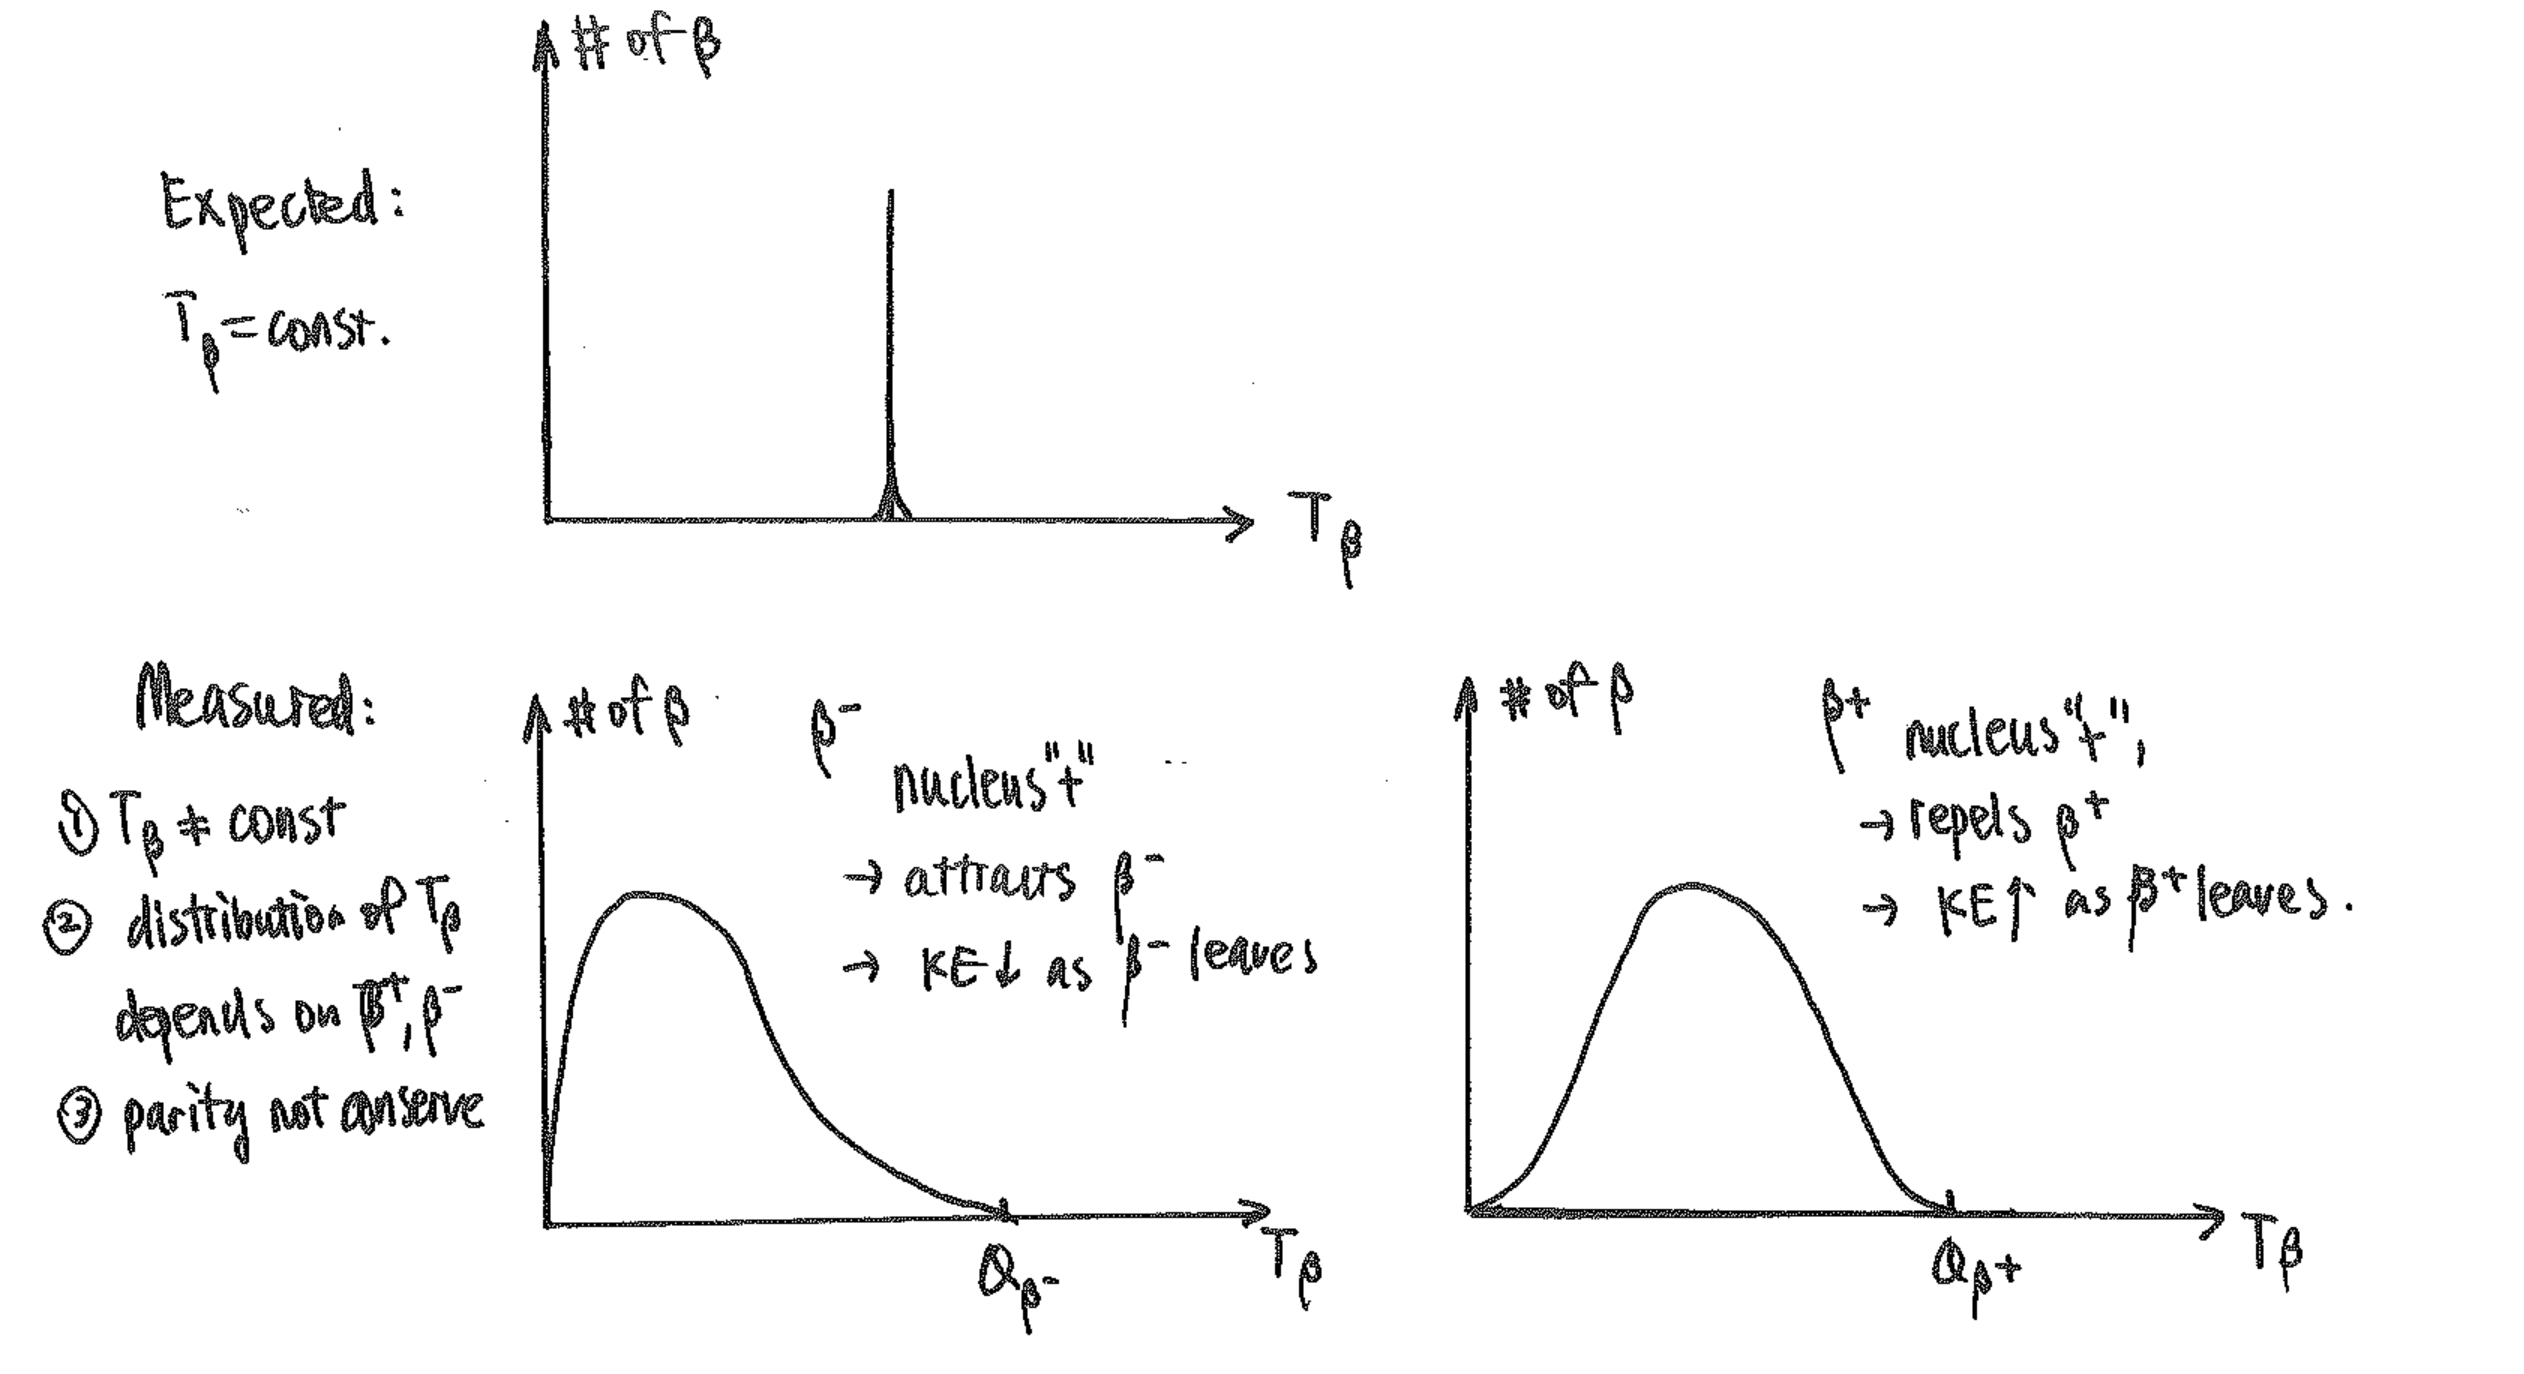
\includegraphics[width=6in]{images/rd/beta-vs-T.png}
    \caption{Expected vs Measured Number of Beta Decays\label{beta-vs-T}}
\end{figure}
\begin{enumerate}
\item $T_{\beta} \neq$ constant. It is a spectrum distribution. After introducing nutrinos, $Q_{\beta}$: $T_{\beta} + T_{\bar{\nu}} = Q_{\beta}, T_{\beta}^{\mathrm{max}} = Q_{\beta}, \expect{T_{\beta}} < Q_{\beta}$. 
\item Electrostatic results: 
    \begin{enumerate}
    \item $\beta^+$: nucleus repels $\beta^+$, KE $\up$.
    \item $\beta^-$: nucleus attracts $\beta^-$, KE $\down$. 
    \end{enumerate}
\item Parity does not conserve yet: \ce{^3H \to \ce{^3He} + e^-}, $\frac{1}{2} \neq 0 \mbox{ or } 1$ (from $ \frac{1}{2} + \frac{1}{2}$).
\item $N(T_{\beta}) \Rightarrow \lambda_{\beta} (E_f)$: number of beta particles is depend on energy; hence decay constant for beta decay is dependent on energy as well.
\end{enumerate}
To explain point 1 \& 3, we introduce neutrino, which are:
\begin{itemize}
\item charge  =0, neutral particles;
\item spin = $\frac{1}{2}$;
\item mass $< \frac{1}{2000} m_e \sim 0 $
\item penetrate easily.  
\item neutrino $\nu$ accompanies $\beta^+$, antineutrino $\bar{\nu}$ accompanies $\beta^-$.
\end{itemize}
The updated beta decays are: 

\ce{^A_Z X_N ->[\beta^-] ^Z_{Z+1} X_{N-1} + e^- + \bar{\nu}};

\ce{^A_Z X_N ->[\beta^+] ^Z_{Z-1} X_{N+1} + e^+ + \nu};

\ce{e + p ->[e.c.] n + \nu}.

The energetics associated with these updated beta decays are (notice $m_n$ is nucleus mass, m is atomic mass; keep in mind $Q>0$ is the criterion for a decay to happen):
\begin{align}
Q_{\beta^-} &= \left[ m_n (\ce{^A_Z X_N}) - m_n (\ce{^A_{Z+1} X_{N+1}}) - m_e \right] c^2 = \left[ m (\ce{^A_Z X_N}) - m (\ce{^A_{Z+1} X_{N}}) \right] c^2 \\
Q_{\beta^+} &= \left[ m (\ce{^A_Z X_N}) - m (\ce{^A_{Z-1} X_{N}}) - 2m_e \right] c^2 \\
Q_{\epsilon} &= \left[ m (\ce{^A_Z X_N}) - m (\ce{^A_{Z+1} X_{N+1}}) \right] c^2 - B_n 
\end{align}


%%%%%%%%%%%%%%%%%%%%%%% Fermi's Golden Rule %%%%%%%%%%%%%%%%%%%%%%%%%
\subtopic{Fermi's Golden Rule}
Fermi's treatment: beta decay is a transition is caused by weak interaction; it depends on the coupling between the initial state $(i)$ and final state $(f)$. Fermi's Golden Rule is:
\begin{align}
\lambda_{if} &= \frac{2\pi}{\hbar} |M_{if}|^2 \rho_f  & \mbox{Transition Probability} &\sim \mbox{Interaction Matrix} \times \mbox{Density of Final States} \\
M_{if} &= \int_{V} \psi_f^* V \psi_i \dV   &  \psi_f &= \mbox{entire final state after decay} = \psi_D \psi_{\beta} \psi_{\nu} \\
P_{if} &= |M_{if}|^2
\end{align}
We will go over the terms:
\begin{enumerate}
\item $\rho_{f}$ is the density of final states available for find $\frac{\derivative n}{\derivative E_f}$ state. $\rho_f$ describes the number of ways the transition can happen. A transition is more likely to occur if there is a large number of accessible final state. $\rho_f$ depends on energy $T_{\beta}$: 
\begin{align}
\rho_f &= \frac{\derivative n}{\derivative E_f} \\ 
\dn_{e} &\propto p_{e}^2  \dpee_{e} & \dn_{\nu} &\propto p_{\nu}^2 \dpee_{\nu} \\
\dn^2 &= \dn_{e} \dn_{\nu} & \frac{\derivative^2 n}{\derivative E_f^2} &\propto p_{e}^2 p_{\nu}^2 \dpee_{e} \dpee_{\nu}  
\end{align}
%
\item $M_{if}$ is the matrix element for the interaction between the initial and final states. It describes the strength of coupling between initial and final states (higher strength $\to$ stronger coupling $\to$ faster transition).$V$ is an operator describing the interaction which causes the transition. The form of $V$ takes another 20 years to find using experimental results for $N(p)$.
\item To future the discussion on $M_{if}$, consider beta and neutrino as free particles. 
\begin{align}
\psi_{\beta} (r) &= e^{i p_{e} r /\hbar} = 1+ \frac{i p_{e} r }{\hbar} + \frac{1}{2} \left(\frac{i p_{e} r }{\hbar} \right)^2 + \cdots \label{beta-wavefunction}\\
\psi_{\nu} (r) &= e^{i p_{\nu} r /\hbar} = 1+ \frac{i p_{\nu} r }{\hbar} + \frac{1}{2} \left(\frac{i p_{\nu} r }{\hbar} \right)^2 + \cdots 
\end{align}
Given $T_{e} = 1 \MeV$, $T_e = \sqrt{p^2 c^2 + m_e^2 c^4} - m_e c^2 \Rightarrow p_{e} = 1.4 \MeV/c^2 \Rightarrow \frac{p_{e}}{\hbar} = 0.007 \fm^{-1} \Rightarrow \frac{p_e r}{\hbar} \ll 1$. With this approximation,
\eqn{ \psi_e (r) \xrightarrow{\frac{pr}{\hbar} \ll 1} 1, \fsp \psi_{\nu} (r) \xrightarrow{\frac{pr}{\hbar} \ll 1} 1 } 
\textcolor{blue}{This yields the `allowed approximation,' similar to S-wave approximation's assumption of $l=0$. This allowed state is the most likely one. The derived results have no $p_e, p_{\nu}$ dependency.}
\end{enumerate}
Let's put everything together\footnote{Krane Eq.9.25}: 
\begin{align}
\dlambda &\propto |M_{if}|^2 p_{e}^2 p_{\nu}^2 \dpee_{e} \left(\frac{\derivative p_{\nu}}{\derivative E_f} \right)^{1/c} \\
N(p_{e}) \dpee_{e} &= A p_{e}^2 p_{\nu}^2 \dpee_{e} \\
N(p_{e}) &= A p_{e}^2 p_{\nu}^2, \fsp \fsp p_{\nu} =\frac{1}{c} (Q - T_{e}) \\
N(p_{e}) &= A p_{e}^2 (Q - T_{e})^2  = A p_{e}^2 \left[ Q - \sqrt{p_{e}^2 c^2 + m_e^2 c^4} + m_e c^2 \right]^2 \\
N(T_{e}) &\propto T_{e}^2 (Q - T_{e})^2
\end{align}

\uline{Correction}: Fermi's theory gives the right range we want: $N(p) = N(T_e) = 0$ at the minimum and maximum $p$ and $T_e$. The proposed shape is right (Figure~\ref{distribution}), except we need to tweak two things: 
\begin{itemize}
\item $N(T_e = 0) \neq 0$ for $\beta^-$. 
\item $\beta^+$'s spectrum appears to be shifted to the right compared with $\beta^-$. 
\end{itemize} 

\begin{figure}
  \centering
  \centering
  \begin{subfigure}[b]{0.45\textwidth}
    \centering
    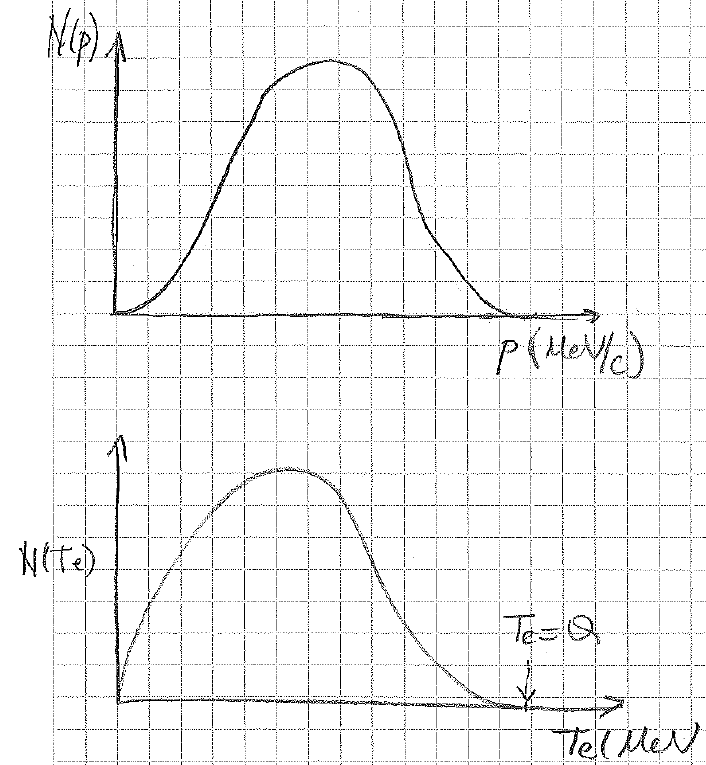
\includegraphics[height=2.7in]{images/rd/beta-predicted-distribution.png}
    \caption{Predicted}\label{beta-predicted}
  \end{subfigure}
  \begin{subfigure}[b]{0.45\textwidth}
    \centering
    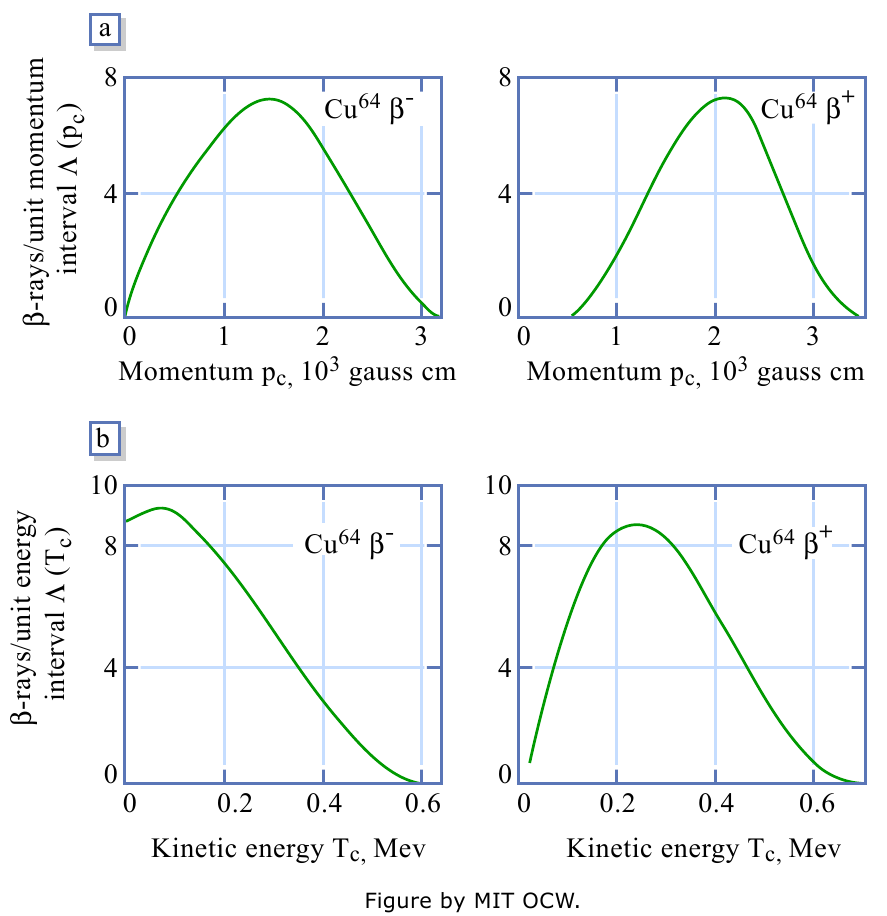
\includegraphics[height=3in]{images/rd/beta-observed-distribution.png}
    \caption{Observed}\label{beta-observed}
  \end{subfigure}
  %\subfloat[Predicted]{\label{beta-predicted}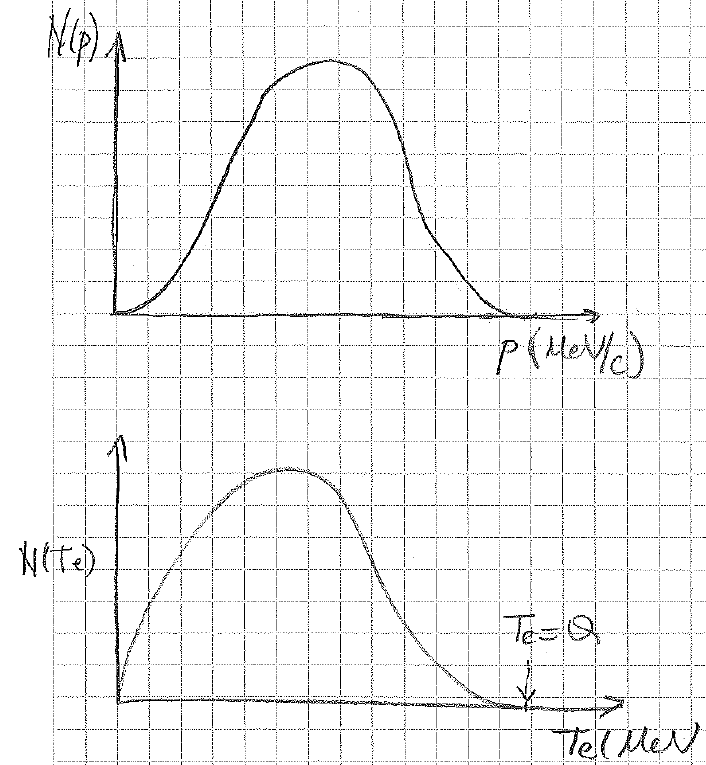
\includegraphics[height=2.7in]{images/rd/beta-predicted-distribution.png}}
  %\subfloat[Observed]{\label{beta-observed}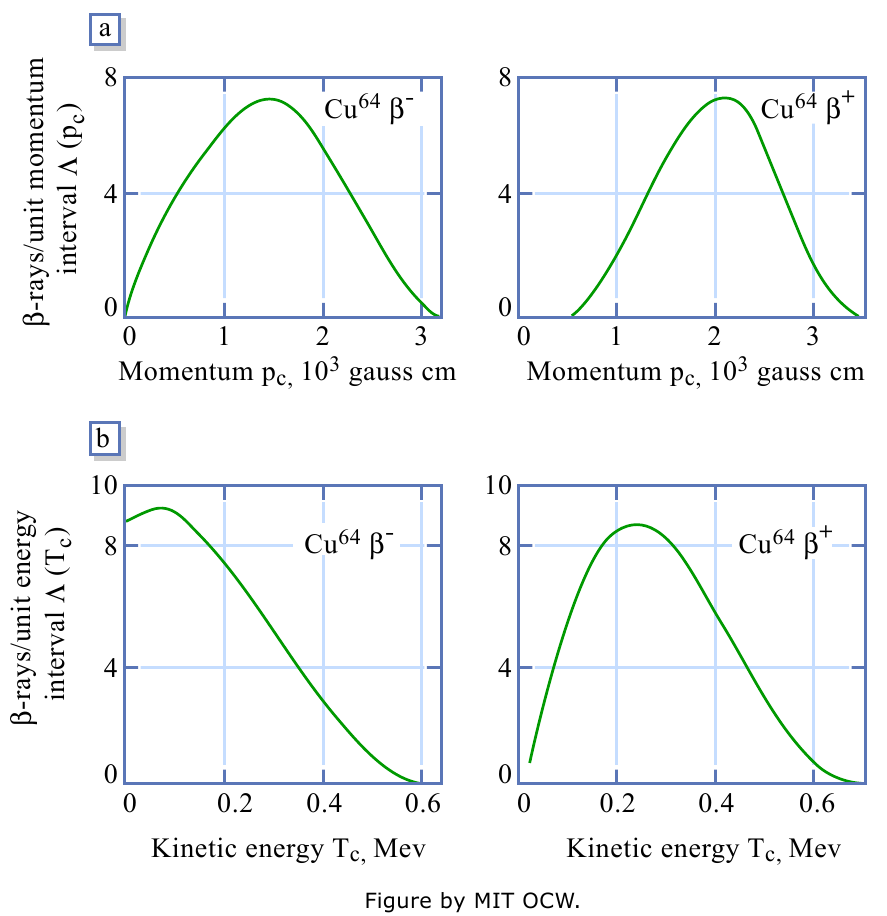
\includegraphics[height=3in]{images/rd/beta-observed-distribution.png}}                  
  \caption{Momentum and Energy Dependency of Neutron Distribution}  \label{distribution}
\end{figure}
Needed correction terms: 
\begin{enumerate}
\item $F(Z^{\prime},p)$ or $F(Z,T_e)$ term (a Fermi function): original model assumes no Coulomb field on $\psi_{\beta}$; we need it to account for Coulomb effect of $\beta^+$ (Coulomb repulsion), $\beta^-$(Coulomb attraction), such that $\beta^+$ would shift the $\beta^-$ spectrum weighted to the right.
\item $S(p_e, p_{\nu})$ term: original model assumes $\frac{pr}{\hbar} \ll 1 \Rightarrow \psi_e \sim \psi_{\nu} \sim 1$, hence no dependence of $M_{if}$ on $p_e, p_{\nu}$. While this assumption is generally valid, it can be wrong sometimes. To correct for it, we need to consider the higher order of $\psi_{\beta}, \psi_{\nu}$ (partial wave). The terms beyond the expansion is commonly called `forbidden decay;' notice they are not absolutely impossible, they are simply with low probability. 
\end{enumerate}
The corrected formula for the distribution of electron momentum (which is proportional to $\lambda(p_e)$) is:
\eqn{N(p_e) = N^o (p_e) \times F(Z^{\prime},p_e) \times S(p_e,p_{\nu}) = C \underbrace{p_e^2 (Q-T_e)^2}_{\textcircled{1}} \underbrace{F(Z^{\prime}, p)}_{\textcircled{2}} \underbrace{|M_{fi}|^2}_{\textcircled{3}} \underbrace{S(p_e, p_{\nu})}_{\textcircled{4}}  }
$\textcircled{1}=$ A statistical factor derived from the density of final states available to the emitted particles; \\
$\textcircled{2}=$ Fermi function to account for the nuclear Coulomb interaction wit the emitted particles;\\
$\textcircled{3}=$ Matrix element for `allowed' ($l_{\beta} = 0$) transition; strength of the interaction between initial and final states; \\
$\textcircled{4}=$ Shape factor to correct $|M_{if}|^2$ for the various `forbidden' transition ($l_{\beta} >0$). 

%%%%%%%%%%%%%%%%% Angular Momentum and Parity %%%%%%%%%%%%%%%%%%
\subtopic{Angular Momentum and Parity Selection Rule}
Nuclear transition must conserve angular momentum and parity, which gives arise to the selection rules below ($I$ is total angular momentum, $L$ is orbital angular momentum, $S$ is spin; subscript $P \sim$ Parent, $D \sim$ Daughter):
\begin{align}
I_P &= I_D + L_{\beta + \nu} + S_{\beta +\nu} \\
\Pi_P &= \Pi_D (-1)^{L_{\beta + \nu}}
\end{align}
\begin{enumerate}
\item The lowest $L$ value corresponds to the most likely state, because $L \down$, $\lambda \up$. Reason: as in Eq.~\ref{beta-wavefunction}, the higher $L$ is, the higher order the expansion is, the less likely the term is, hence we consider the $L=l$ term as l-th forbidden (if $L=0$, we call it allowable). 
\item $\lambda_{\beta} = \lambda (L=0) + \lambda (L=1) + \cdots$, in which $\lambda_{\mathrm{allowed}} \gg \lambda_{\mathrm{forbidden}}, t_{1/2,\mathrm{allowed}} \ll t_{1/2,\mathrm{forbidden}}$. Beta decay's $t_{1/2}$ range from milliseconds to $10^{16}$ years because of the ease in undergoing decay when $l=0$, and the difficulty in doing so when $l>0$. 
\item $S$ can be 0 or 1 (because $S_e = S_{\nu} = \frac{1}{2}$); $S = 0$ is called Fermi decay (F); $S=1$ is called Gamow-Teller decay (G.T.).
\end{enumerate}
Examples:
\begin{itemize} 
\item \ce{^{14}_8 O_6 \to ^{14}_7 N_7^*}. 
    \begin{itemize} 
    \item Spin: $0^+ \to 0^+$, that is, $+ = + (-1)^{L_{\beta + \nu}} \Rightarrow L_{\beta + \nu} = $ even. 
    \item $ 0 = 0 + L_{\beta + \nu}+ S_{\beta + \nu}$. We can have: $(L, S) = (0,0), (1,1)$. From the requirement of the last bullet point, $S=0$ is called the Fermi transition, $L=0$ is the `allowed' one; whereas $L=1$ is the 1st forbidden.  
    \end{itemize}
\item \ce{^{10}_4 Be_6 \to ^{10}_5 B_5}, $3^+ \to 0^+$
    \begin{itemize}
    \item $+ = +^L$, L is even;
    \item $3 = 0 + L + S$. $L = 0$ does not work; $L = 2$ is possible with $S=1$, $L = 2$ is called the 2nd forbidden. 
    \end{itemize}
\item \ce{^{115} In \to ^{115} Sn}, ($\frac{9}{2}^+ \to \frac{1}{2}^+ $)
    \begin{itemize}
    \item $+ = + (-1)^L$, L is even;
    \item $\frac{9}{2} = \frac{1}{2} + L + S$: L cannot be 0 or 2. $L =4,$ S can be either 1 or 0. $L = 4$ is the 4th forbidden, and $S = 1, 0$ are the Fermi and something-else transition. 
    \end{itemize}    
\end{itemize}

\end{document}
